\begin{figure}[h]
    \centering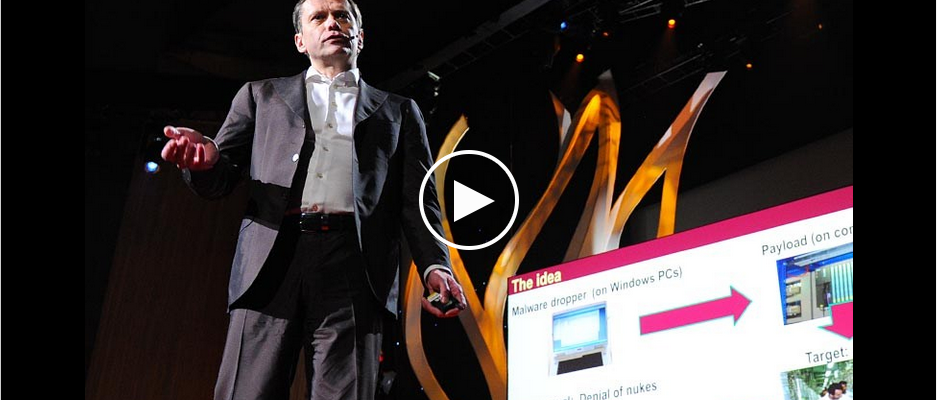
\includegraphics[scale=0.5]{stuxnet.png}
    \caption{\url{http://www.ted.com/talks/ralph\_langner\_cracking\_stuxnet\_a\_21st\_century\_cyberweapon}}
\end{figure}
Compromised systems that controlls centrifuges. Targeted Nucelar engineers.
that works on the systems. Payload is very complex. Looks for system calls, 
because their behaviour is know, Looks for timers and data structures. Smaller
payload seems designed to slowly crack centrifuge rotors. Big payload 
manipulates valves. Intercepts values from sensors, and gives fake input data. 
The idea is to circumvent digital safety systems. For more information on 
Stuxnet see:\\
\begin{enumerate}
    \item \url{https://en.wikipedia.org/wiki/Stuxnet}
    \item \url{https://archive.today/WS5uA}
    \item \url{http://go.eset.com/us/resources/white-papers/Stuxnet\_Under\_the\_Microscope.pdf}
    \item \url{http://www.symantec.com/content/en/us/enterprise/media/security\_response/whitepapers/w32\_stuxnet\_dossier.pdf}
\end{enumerate}

\textit{Digital evidence, evidence integrity and evidence dynamics}. 
We define digital evidence as any digital data that contains reliable 
information that supports or refutes a hypothesis about an incident.
Evidence integrity refers to the preservation of the evidence in its original 
form. This is a requirement that is valid both for the original evidence and the
image. Evidence dynamics is described to be any influence that changes, 
relocates, obscures, or obliterates evidence, regardless of intent.

\textit{Chain of custody and forensic soundness} - Chain of custody refers to 
the documentation of evidence acquisition, control, analysis and disposition 
of physical and electronic evidence. The term forensically sound methods and 
tools usually refers to the fact that the methods and tools adhere to best 
practice and legal requirements.

\textit{OOV} - Collect the most volatile data first – this increases the 
possibility to capture data about the incident in question. BUT: As you capture 
data in one part of the computer, you’re changing data in another

\textit{Evidence acquisition and verification} - For digital forensics it is typically
copy the data to a secure store, and then verify that the copy is
identical.

\textit{Cybercrime convention} - International agreement to increase cooperation
between countries. Criminal Law so things should be illeagal in all
countries. Criminal Procedure law, what police can do and how they do it.
Internet is borderless so there needs to be a effective cooperation
between countries to catch the bad guys.

\textit{Uncertanties in internet tracing} - Traffic is routed, so you do not
know if is original, anon traffic, time limits. TOR, VPN, proxies etc.

\subsection{File System Forensics}
\begin{figure}[h]
    \centering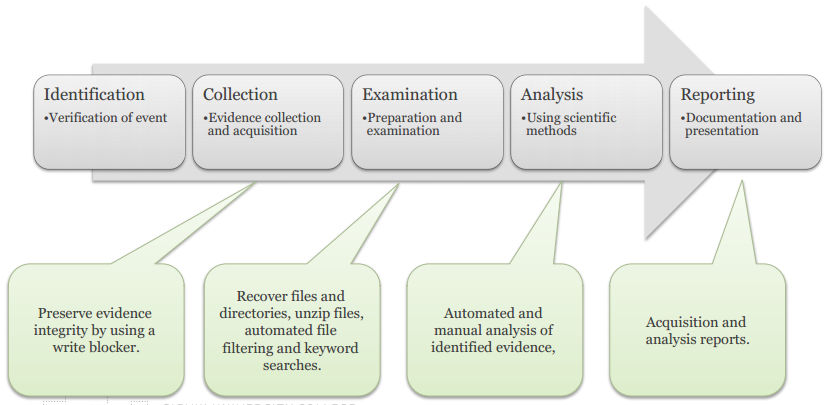
\includegraphics[scale=0.5]{fs_forensics.png}
\end{figure}
\begin{figure}[h]
    \centering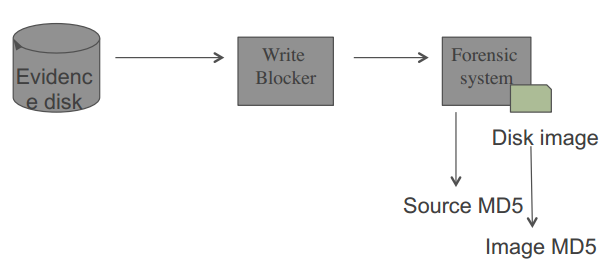
\includegraphics[scale=0.5]{disk_img.png}
\end{figure}

Forensic soundness and evidence integrity are critical, if a disk is found that
you belive contains evidence you need to make sure that any copy is forensically
sound, and the integrity of the evidence is preserved. To do this you connect
the disk to a write blocker. Write blockers are devices that allow acquisition 
of information on a drive without creating the possibility of accidentally 
damaging the drive contents. They do this by allowing read commands to pass but 
by blocking write commands, hence their name.\\

There are two ways to build a write-blocker: the blocker can allow all commands 
to pass from the computer to the drive except for those that are on a particular
list. Alternatively, the blocker can specifically block the write commands and 
let everything else through.\\

Write blockers may also include drive protection which will limit the speed of a
drive attached to the blocker. Drives that run at higher speed work harder(the 
head moves back and forth more often due to read errors). This added protection 
could allow drives that can not be read at high speed (UDMA modes) to be read at 
the slower modes (PIO).\\

There are two types of write blockers, Native and Tailgate. A Native device uses 
the same interface on for both in and out, for example a IDE to IDE write block. 
A Tailgate device uses one interface for one side and a different one for the 
other, for example a Firewire to SATA write block.
\footnote{http://www.forensicswiki.org/wiki/Write\_Blockers}\\

Hardware write blockers can be either IDE-to-IDE or Firewire/USB-to-IDE. 
Simson prefers the IDE-to-IDE because they deal better with errors on the drive 
and make it easier to access special information that is only accessible over 
the IDE interface.\\

Software write blockers can be either tailored to an individual operating system
or can be an independent boot disk. Their main upsides are with ease of use, 
since they are on a CD and do not require you to open up the case, and speed 
since they do not become a bottle neck.\\




    Media Analysis
    Hard drives.
    Technologies :Magnetic, SSD
    SSD are much more difficult for digital forensics, deleted data may dissappear compared
    to magnetic drives where the deleted data can persist for a long time
    untill it is overwritten.

    Many interfaces; SATA; PATA, SCSI, ATA/IDE

    Disk encryption much more common today, requiers live forensics if
    you do not have password. If the computer is turned of your shit out of
    luck.
    
    HPA capeable to block OS accessing the harddrive.
    External media as well, and cloud services.


    Layers of abstraction
    Timestamps are gold mines for establishing time lines.

    DOS Partitions
    512 first bytes are the MBR, each partition can have a MBR

    A block is either allocated or not. Unallocated may contain data
    even if they are not used.
    Slackspace can be found at the end of sectors or block, it occurs
    when a file does not fill the end of the sector or block, and may
    contain data from old files.

    Type 1 SS is the unused part of a sector, Type 2 is a unused block
    in a cluster.

    Slackspace and unallocated blocks are sources for deleted data.

    FAT boot sector
    name of os
    sectors per cluster
    Max number of root dir entries
    volume name
    serial number

    NTFS has more info
    
    FAT directory entries
        filename
        long filename
        MAC times (creation modification acces)
        file size
        first cluster number

    NTFS Master file table entries
        stadard information
        file name
        data
    
    Windows delete files
    Fat: File name minus first letter is perserved, MAC perserved
    cluster will be marked as unalloced, but the data is perserved.

    NTFS: File name and MFT number preserved,
    MAC times perserved and used clusters will be marked as un allocated.

    bottom line, everything is there.
    For magnetic disk this is importaint

    UNIX
    file systems are organized within a single tree structure
    underneath one root directory.
    Disk partition are mounted at some directory in the file
    system tree.

    UNIX file types:
    regular files
    directories
    symbolic lincs
    IPC endpoints
    Device files

    Metadata is stored in inode blocks
    Unix file deletion
    The dir entry and inode block are unallocated
    MAC time stamps are changed, so that information is lost
    All other data is preserved.

    MAC OS
    HFS+
    Volume header
    allocation blocks
    Allocation file
    Catalog file

    5 time stamps
    Created
    Content Mod
    Attribute Modified
    Accessed
    Backed Up - If it recent it tells you that it is likely backed up.

    SSD disks
    SSDS are non volatile
    Blocks are subdivided into pages
    Cannot delete - no standard way to overwrite all blocks, only
    about 80% of the isk is actually available.
    Cannot recover - "dirty" blocks are erased
    Self corrosion (Garbage Collection) - SSD writes over unused blocks
    Model dependent, especially older SSDs may not do this.

    Case, in class discussion
    % Copy paste from slides

\subsection{Live Forensics}
    Considerations:
        OOV - If you want data in memory you need to do live forensics.
        
        Storing evidence remotely - If evidence is on network shares or
        in the cloud

        Using trusted tools - When dealing with compromised systems you 
        cannot trust the systems tool, you need to bring external tools.

    Motivation:
        System subversion - Hacked systems, a lot of information will be
        in the system state such as network stack and memory.

        Encryption and passwords - You need to do live forensics, if it
        is shut down and you do not know the password then you need to do it
        live

        Running applications - Text in documents that are not saved

        Open network connections - Investigating p2p networks you will want
        to know which other computers it is talking too.

\begin{figure}[h]                                                                                                                 
    \centering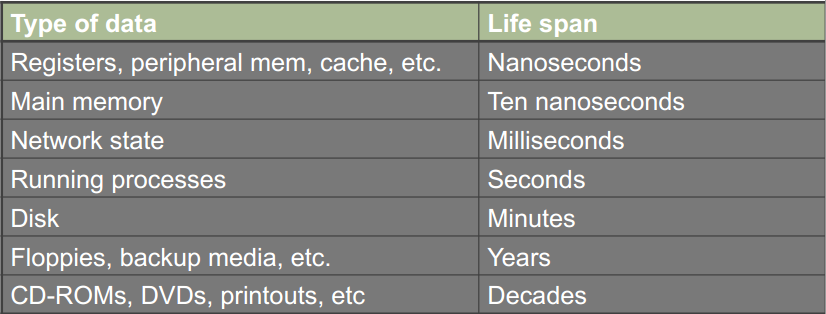
\includegraphics[scale=0.5]{oov.png}
    \caption{Table showing the life time of the different data types}
\end{figure}

    OOV  expected lifetime of data table.

    WHich order
        Memory dump

        Process info
        Network info
        File MAC times
        File system

    if you choose one the other will deteriorate. 

    A rootkit can alter the data from process and system status tools.
    Rootkits
    Command level rootkits hide their presence through changing system
    commands.

    Library level rootkits hide their presence through changing system run time
    libs

    Kernel level rootkits hide their presence through changing the system
    kernel.

    Computer Memory
    Memory can be found in many sources, RAM swap space Hibernation files.

    Memory analysis
    Fragments of files can be found by searching for hashes.

\subsection{Remote Foresincs}
    Get data a from a remote computer.
    Think about secure channels, not good to copy thing in plaintext
    over the net.


